%%%%%%%%%%%%%%%%%%%%%%%%%%%%%%%%%%%%%%%%%%%%%%%%
%%%%%%%%%%%%%%%%%%%%%%%%%%%%%%%%%%%%%%%%%%%%%%%%
%
%		Kommentar
%		Ein nettes old school template.......
%		last modified: 27/03/07
%
%%%%%%%%%%%%%%%%%%%%%%%%%%%%%%%%%%%%%%%%%%%%%%%%
%%%%%%%%%%%%%%%%%%%%%%%%%%%%%%%%%%%%%%%%%%%%%%%%
\documentclass[a4book,11pt,twoside]{scrbook}
\usepackage{eurosym}
\usepackage[german]{babel}
\usepackage{amsmath}
\usepackage{amssymb}
\usepackage[automark]{scrpage2}	%Kopfzeile Autoinhalt (Kapitel)
\usepackage{graphics}
\usepackage{color}
\usepackage{graphicx}
\usepackage{longtable}
\usepackage{lscape}
\usepackage{hhline}
\usepackage{booktabs}
\usepackage{IFSlogo}
% \usepackage[T1]{fontenc}
% \usepackage[pdftex]{hyperref}
\usepackage{makeidx}
\selectlanguage{german}
\setlength{\parindent}{0pt}  % setzt sie Einrückung nach einem Umbruch zurück

%%%%%%%%%%%%%%%%%%%%%%%%%%%%%%%%%%%%%%%%%%%%%%%%
%		Sachregister-Erstellung
%		Begriffe werden mit Befehl \index{} aufgenommen
% 		Index erstellen in Konsole makeindex -g -s style.ist Vorlage.idx 
%%%%%%%%%%%%%%%%%%%%%%%%%%%%%%%%%%%%%%%%%%%%%%%% 
\makeindex


%%%%%%%%%%%%%%%%%%%%%%%%%%%%%%%%%%%%%%%%%%%%%%%%
%		ETH-Schrift einführen
%%%%%%%%%%%%%%%%%%%%%%%%%%%%%%%%%%%%%%%%%%%%%%%% 

\usepackage[standard-baselineskips]{cmbright} % Mathematikschrift die in etwa ETH-Light entspr.
\renewcommand{\sectfont}{\bfseries}

%\renewcommand{\familydefault}{let} 
%\renewcommand{\seriesdefault}{let}
%\renewcommand{\shapedefault}{let}
%\renewcommand{\sfdefault}{let}
\renewcommand{\rmdefault}{let}


% \DeclareFixedFont{\x}{T1}{let}{m}{n}{10}
% \DeclareFixedFont{\xb}{T1}{let}{m}{n}{10}
% \newfont{\xiiiv}{letr8t at 8.0pt}
% \newfont{\xiiivb}{letb8t at 8.0pt}


%%%%%%%%%%%%%%%%%%%%%%%%
% Schriftengefrickel
%%%%%%%%%%%%%%%%%%%%%%%%%
\usepackage{fontspec}
\usepackage{sectsty}

\partfont{\font \x="DINNeuzeitGroteskStd-Light" at 40pt\x}
\chapterfont{\font \x="DINNeuzeitGroteskStd-Light" at 32pt\x}
\sectionfont{\font \x="DINNeuzeitGroteskStd-Light" at 16pt\x}
\subsectionfont{\font \x="DINNeuzeitGroteskStd-Light" at 14pt\x}
\subsubsectionfont{\font \x="DINNeuzeitGroteskStd-Light" at 14pt\x}
\paragraphfont{\font \x="DINNeuzeitGroteskStd-Light" at 14pt\x}
\newfontface\swashed[Contextuals=Swash, Ligatures=Common]{Adobe Garamond Pro Italic}
\newfontface\foo[Numbers={OldStyle},Contextuals=Swash, Ligatures=Common]{Adobe Garamond Pro}
\newfontface\foofat[Numbers={OldStyle},Contextuals=Swash, Ligatures=Common]{Adobe Garamond Pro Bold}


\usepackage[a4paper,left=4.0cm, right=4.0cm,top=3.0cm, bottom=3.0cm]{geometry}
	
%%%%%%%%%%%%%%%%%%%%%%%%%%%%%%%%%%%%%%%%%%%%%%%%
%		eigenen Stil definieren
%%%%%%%%%%%%%%%%%%%%%%%%%%%%%%%%%%%%%%%%%%%%%%%% 
\pagestyle{scrheadings}
\renewcommand*{\chapterpagestyle}{scrheadings} 
\clearscrheadfoot 
\ihead{\textsf{\headmark}} 
\ohead{\pagemark}
\setheadsepline{.4pt}
\setfootsepline{.4pt}
\ifoot{}
\ofoot{\footnotesize{\textsc{Hsr, Silvio Heuberger}}}


% frickelabst�nde

% abst�nde und sooooo
\setlength{\columnsep}{10mm}
\setlength{\parskip}{2.5mm}

%two column float page must be 90% full
\renewcommand\dblfloatpagefraction{.90}
%two column top float can cover up to 80% of page
\renewcommand\dbltopfraction{.80}
%float page must be 90% full
\renewcommand\floatpagefraction{.90}
%top float can cover up to 80% of page
\renewcommand\topfraction{.80}
%bottom float can cover up to 80% of page
\renewcommand\bottomfraction{.80}
%at least 10% of a normal page must contain text
\renewcommand\textfraction{.1}


%%%%%%%%%%%%%%%%%%%%%%%%%%
% listings for everyone

\definecolor{defgray}{cmyk}{0.3,0.05,0,0.43}
\usepackage[plainpages={false}, bookmarks, pdfstartview={FitV}, colorlinks, linkcolor=defgray]{hyperref}


\usepackage{listings}
\lstset{% general command to set parameter(s)
basicstyle=\ttfamily\small, % print whole listing small
%basicstyle=\small,
commentstyle=\color{defgray}, % comments
stringstyle=\ttfamily, % typewriter type for strings
showstringspaces=false,
keywordstyle=\bfseries\color{blue},
numbers=left,
numberstyle=\color{defgray}\tiny,
frame=single,
%frame=shadowbox,
%frameround=tttt,
rulesepcolor=\color{defgray},
language={ruby}
} % no special string spaces


% make monospace font the same size (optocally) as Arno Pro
\setmonofont[Scale=0.9]{ITC American Typewriter Std Condensed}
\defaultfontfeatures{Scale=MatchLowercase,Mapping=tex-text}


\begin{document}
\renewcommand{\theequation}{\thesection.\arabic}
\addtokomafont{caption}{\small}
\setkomafont{captionlabel}{\sffamily\bfseries}
\numberwithin{equation}{section}
\pagenumbering{Roman}
\setcapindent*{1em}

%%%%%%%%%%%%%%%%%%%%%%%%%%%%%%%%%%%%%%%%%%%%%%%%
%		Titelseite
%%%%%%%%%%%%%%%%%%%%%%%%%%%%%%%%%%%%%%%%%%%%%%%%
\titlehead{
	\begin{minipage}{0.6\textwidth}{\IFSlogo[50mm]}
 	\end{minipage}
	\begin{minipage}{0.4\textwidth}
		\footnotesize \rightline{HSR Rapperswil} \rightline{Institut für Software}
	\end{minipage}
 } 

\author{Silvio Heuberger \\ Institut für Software}
\subject{Lecture Notes}
\title{Ruby, code-driven}
\date{FS 2009}
\publishers{}
\dedication{} 
\maketitle



\tableofcontents

\fontspec[Numbers={OldStyle}, Ligatures={Common}]{Adobe Garamond Pro}

\chapter{Ruby? Noch eine Sprache?} % (fold)
\label{cha:ruby_noch_eine_sprache_}

\pagenumbering{arabic}
\section{Was macht Ruby so speziell?} % (fold)
\label{sec:was_macht_ruby_so_speziell_}
Ruby ist eine spezielle Programmiersprache. Speziell für Programmierer, die sich statisch typisierte Sprachen wie Java, C\# und C++ gewöhnt sind. Folgende Punkte zeichnen Ruby aus:

\subsection*{Ruby ist einfach zu lesen} % (fold)
\label{sub:ruby_ist_einfach_zu_lesen}

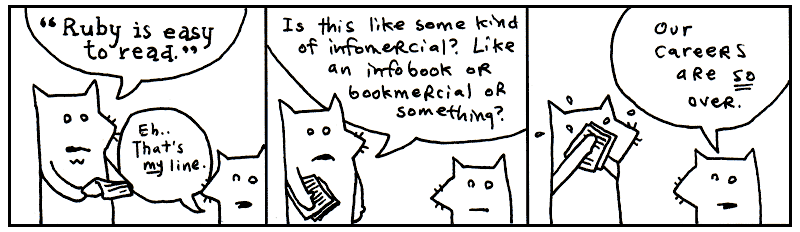
\includegraphics[width=\textwidth]{img/easy_to_read.png}

Lies folgenden Code laut vor:
\lstinputlisting{code/easytoread.rb}

Ruby ist »Coderspeak«, nicht nur eine Programmiersprache. Das obige Programm tut genau das, was erwartet wird, wenn man den Code vorliest.

Ein weiteres Beispiel ist folgender Code:
\lstinputlisting{code/easytoread2.rb}

Der Code beendet das Programm, ausser wenn der String »Restaurant« als Teil »aura« enthält, was auch der Fall ist. Ruby nutzt geschickte \emph{Konventionen}, was die Methodennamen angeht um die Lesbarkeit des Codes zu verbessern. Eine Methode, die am Ende des Names ein Fragezeichen hat, ist eine Ja/Nein-Frage an das Objekt auf dem sie aufgerufen wird (also eine Methode die einen \texttt{boolean} als Rückgabewert hat).

Das soll nicht heissen, dass Code der in einer anderen Sprache geschrieben ist schwer zu lesen ist. Vielfach ist das allerdings so und die Konventionen in Ruby machen viele Teile des Codes einfacher zu lesen und befreien ihn von Überraschungen. Mehr dazu im Kapitel \ref{cha:die_syntax_von_ruby}.
% subsection ruby_ist_einfach_zu_lesen (end)



\subsection*{Alles ist ein Objekt} % (fold)
\label{sub:alles_ist_ein_objekt}
In Ruby ist alles ein Objekt. Wirklich alles --- es gibt in Ruby keine Unterscheidung zwischen »primitiven Datentypen« und »benutzerdefinierten Typen«.
Nachfolgend ein paar Beispiele von Methoden, die auf Instanzen von Klassen aufgerufen werden. Nachgestellt als Kommentar ist jeweils das Resultat eines Statements.
\lstinputlisting{code/objects.rb}
% subsection alles_ist_ein_objekt (end)



\subsection*{Duck-Typing} % (fold)
\label{sub:duck_typing}
\begin{quotation}\swashed{\Huge“\normalsize When I see a bird that walks like a duck and swims like a duck and quacks like a duck, I call that bird a duck.\Huge”\normalsize – James Whitcomb Riley}
\end{quotation}

Duck-Typing bedeutet dass erst zur Laufzeit überprüft wird, ob ein Objekt über bestimmte Merkmale — wie zum Beispiel Methodennamen und Attribute — verfügt, was zu einer erhöhten Flexibiltät führt. Es wird aber auch die Möglichkeit reduziert, Typen zur Compile-Zeit statisch zu prüfen und solche Fehler im Programm zu finden.

Hier einfach noch kurz ein Stück Code, das aufzeigt, wie flexibel und doch ausdrucksstark Code mit Duck-Typing werden kann. Über die Syntax mache man sich hier noch nicht allzu viele Gedanken...

\lstinputlisting{code/ducks.rb}

Folgendes gilt für obigen Code:
\begin{itemize}
	\item Vögel haben einen Namen.
	\item Enten sind auch Vögel, darum haben auch sie einen Namen.
	\item Enten haben eine Methode \texttt{quack()}, bei der sie ein entenartiges Geräusch von sich geben.
	\item Die Codezeile 17 iteriert über alle Vögel in \texttt{birds} und falls \texttt{bird.respond\_to? :quack} dann wird diese Methode aufgerufen. Andernfalls ist der Vogel keine Ente.
\end{itemize}

Die Ausgabe des Programms ist dann also:

\begin{lstlisting}
Gustav is not a duck!
Donald: quack!
\end{lstlisting}

Code wie der obige lässt sich mit \texttt{instanceof()} auch noch relativ kurz und prägnant in Java schreiben. Er wird aber schnell einiges komplizierter. Mehr dazu aber später.
% subsection duck_typing (end)



\subsection*{Noch viel mehr!} % (fold)
\label{sub:noch_viel_mehr_}
Dies ist nur ein ganz kleiner Ausschnitt, noch viel mehr macht Ruby zu einer speziellen, attraktiven Programmiersprache. Darauf wird aber erst in nachfolgenden Kapiteln eingegangen. Jetzt noch eine kurze Buzzword-Zusammenfassung, was Ruby so alles kann...
% subsection noch_viel_mehr_ (end)
% section was_macht_ruby_speziell (end)




\section{Woher kommt Ruby und was ist das Ziel (Buzzword Bingo)} % (fold)
\label{sec:woher_kommt_ruby_und_was_ist_das_ziel}
Ruby wurde von Yukihiro »Matz« Matsumoto in Japan im Jahre 1995 zum ersten Mal released. Weltweit erreichte die Sprache danach den Ruf einer einfach zu erlernenden, mächtigen und expressiven Sprache.
Die Intention war damals ein »Perl, better than Perl« als Sprache zu entwerfen.

Folgende Kernpunkte sollten Ruby auszeichnen:
\begin{itemize}
	\item Pure OO-Sprache
	\item Simpel und frei von Überraschungen
	\item Mächtige und flexible Sprache
	\item Produktiv: Schnelle Entwicklung
	\item Nicht kommerziell: Ruby ist Open-Source
	\item Robust: Ruby hat einen Garbage-Collector
	\item Flexibel: Dynamisch typisierte Sprache
\end{itemize}
% section woher_kommt_ruby_und_was_ist_das_ziel (end)






% chapter ruby_noch_eine_sprache_ (end)

\chapter{Die Syntax von Ruby} % (fold)
\label{cha:die_syntax_von_ruby}
Die Syntax von Ruby ist kurz, prägnant und sprechend. Ruby wurde bewusst als »sprechbare« Sprache designt. Wenn eine Sprache der natürlichen Sprache ähnelt, so ist sie auch einfacher zu lesen und verstehen.
% chapter die_syntax_von_ruby (end)





\section{Variablen} % (fold)
\label{sub:variablen}
Variablennamen in Ruby bestehen aus Kleinbuchstaben, Zahlen und Underscores, dürfen aber nicht mit einer Zahl anfangen. Variablen können direkt einen Wert zugewiesen bekommen.

Normalerweise werden Variablennamen in Ruby nicht in CamelCase geschrieben, wie das in Java oder C der Fall ist, sondern mit Underscores zusammengehängt. Solche Style-Guidelines können aber zum Beispiel für ein gesamtes Projekt geändert werden, wobei man der Opensourcewelt eine Freude macht, wenn man sich daran hält...

Gültige Beispiele wären:
\lstinputlisting{code/variables.rb}
% section variablen (end)






\section{Zahlen} % (fold)
\label{sec:zahlen}
Die einfachsten Zahlen sind Ganzzahlen (\texttt{Integer}). Diese bestehen in Ruby aus einer beliebig langen Folge — richtig gelesen, Ruby hat automatischen Support für grosse Zahlen mit hunderten von Stellen — von Ziffern mit vorgestelltem Minus- oder Pluszeichen.

Fliesskommazahlen werden mit einem Dezimalpunkt geschrieben. Auch die wissenschaftliche Notation wird unterstützt.

\lstinputlisting{code/numbers.rb}
% section zahlen (end)






\section{Strings} % (fold)
\label{sec:strings}
Strings in Ruby kommen in verschiedenen Quote-Gewändern.
\begin{enumerate}
	\item Double-Quoted
	\item Single-Qouted
	\item General Delimited, dabei wird nach \% ein Character angegeben, mit dem der Anfang und das Ende des Strings markiert ist. Klammern sind auch möglich.
\end{enumerate}

Folgender Code illustiert das:
\lstinputlisting{code/strings.rb}

Diese Strings werden dann wie angegeben ausgegeben (Code bis Zeile 8).

In Strings können auch mit der speziellen Zeichenfolge \#\{[Variable]\} Werte von Variablen eingesetzt werden.

% section strings (end)




\section{Symbols} % (fold)
\label{sec:symbols}
Symbols sind ein spezielles Element von Ruby, verglichen mit anderen Sprachen. Ein Symbol ist genau gleich wie ein Variablenname/String definiert, sie fangen aber mit \emph{einem Doppelpunkt} an.

Symbols sind \emph{leichtgewichtige} Strings. Ein bestimmter Name für ein Symbol erzeugt immer das gleiche Symbol, egal wie oft es im Sourcecode vorkommt.

Als Vergleich: Ein String-Literal (auch in Java) erzeugt \emph{immer} ein neues String-Objekt. Normalerweise verwendet man Symbols dort, wo ein String gebraucht wird, der aber nie auf dem Screen ausgegeben wird, wie zum Beispiel Namen von Methoden oder Hash-Elementen. (Siehe auch das Beispiel zu Duck-Typing)

\lstinputlisting{code/symbols.rb}
% section symbols (end)






\section{Konstanten} % (fold)
\label{sec:konstanten}
Konstanten werden in Ruby geschrieben wie Variablen, fangen aber mit einem \emph{Grossbuchstaben} an. Wenn versucht wird den Wert einer Konstanten zu ändern, so funktioniert das zwar, aber Ruby zeigt uns eine Warnung, dass wir gerade eine bereits initialisierte Konstante geändert haben.

Konstanten sollte man besser nicht ändern!

\lstinputlisting{code/constants.rb}

Wird dieser Code ausgeführt, so zeigt sich Ruby nur mässig erfreut — der Code läuft aber weiter:
\begin{lstlisting}
/dev/keyboard0
constants.rb:2: warning: already initialized constant File_Location
\end{lstlisting}
% section konstanten (end)





\section{Parallele Zuweisung von Variablen}
Ruby unterstützt die parallele Zuweisung von Variablen. Das ermöglicht zum Beispiel die Funktion \texttt{swap(a,b)} für zwei Elemente ganz elegant zu schreiben:

\lstinputlisting{code/swap.rb}

Weiter können auch mehrere Variablen elegant und kurz auf Standardwerte gesetzt werden. Die \emph{kann} die Lesbarkeit erhöhen, kann aber auch am falschen Ort benutzt werden.

\lstinputlisting{code/parallel.rb}






\section{Methoden} % (fold)
\label{sec:methoden}
Methoden in Ruby werden durch einen '.' an eine Variable oder Konstante angehängt. Es gilt die Konvetion, dass Methoden die einen \texttt{boolean} zurückliefern am Ende ihres Namens ein '?' tragen. Methoden, die ein Objekt direkt verändern und nicht eine Kopie eines veränderten Objektes zurückgeben, tragen ein '!' am Ende ihres Namens.

Die Klammern können in Ruby in vielen Fällen weggelassen werden, was je nach Situation die Lesbarkeit des Codes erhöht.

\lstinputlisting{code/methods.rb}

Der Methodenaufruf auf Zeile 1 gibt ein neues \texttt{Door}-Objekt zurück das geöffnet ist. \texttt{open!} öffnet direkt die Türe auf der die Methode aufgerufen wurde.

Diese Notation wird dann wichtig, wenn Methode der Ruby-Library verwendet werden, wo es oft zwei Versionen einer Methode gibt — eine mit '!' und eine ohne.
% section methoden (end)







\section{Klassen, Attribute} % (fold)
\label{sec:klassen_methoden_attribute}
Gleich ein Beispiel einer Klasse in Ruby:

\lstinputlisting{code/song.rb}

Dieses Beispiel zeigt gleich einige Aspekte auf, wie in Ruby eine Klasse geschrieben wird:

\begin{enumerate}
	\item \texttt{attr\_accessor} generiert Getter und Setter für Properties. (Und nimmt als Werte offenbar Symbols gerne entgegen...)
	\item Man kann Getter und Setter auch als Methoden schreiben. Siehe \texttt{minutes=} und \texttt{minutes}.
	\item Instanzvariablen fangen mit einem '@' an.
	\item Klassenvariablen mit '@@'.
	\item Wir können ein Property, das einen Setter hat einfach mit '=' zuweisen.
	\item Das \texttt{return}-Statement ist optional, da der letze Wert in der Funktion zurückgegeben wird. Dies ist nur bei \emph{kurzen} Methoden sinnvoll.
\end{enumerate}

Alle Klassen in Ruby sind \emph{offen} für Erweiterung, was sehr praktisch sein kann und den Code kürzer macht, weil nicht für jedes Feature eine neue Klasse geschrieben werden muss, wenn die Funktion in eine andere Klasse \emph{gehört}.

\lstinputlisting{code/prime.rb}

Dies sollte man aber nicht tun — auch wenn man kann:

\lstinputlisting{code/plusminus.rb}
% section klassen_methoden_attribute (end)



\section{Module und Mixins} % (fold)
\label{sec:module_und_mixin}
Im Gegensatz zu anderen objektorientierten Sprachen unterstützt Ruby nur die einfache Vererbung. Dafür kennt Ruby \emph{Module}. Module sind an sich Sammlungen von Funktionen und Klassen können dann Module als Mixin verwenden und bekommen dadurch ihre Methoden geschenkt. Zusammen mit Duck-Typing ergibt sich ein sehr flexibles Konzept.

Interessant wird das Ganze, wenn der Code aus dem Modul Code aus der Klasse verwenden kann um neue Methoden zu definieren.

So kann eine Klasse, welche die Methode \texttt{each} definiert das Modul \texttt{Enumerable} einmixen und erhält so etwa 20 Methoden \emph{gratis}. Darunter auch besonders nützliche wie:
\begin{itemize}
	\item \texttt{find}
	\item \texttt{find\_all}
	\item \texttt{include?}
	\item \texttt{collect}
	\item \texttt{sort}
\end{itemize}
% section module_und_mixin (end)


\section{Blocks und Closures} % (fold)
\label{sec:blocks_und_closures}
Blöcke sind ein essentieller Teil der Sprache Ruby. Code in geschweiften Klammern ist ein Block. Allerdings ist ein Block mehr als nur Code der gruppiert ist.

Ein Block wird in Ruby eigentlich immer zusammen mit einer Methode verwendet. Damit kann man zum Beispiel Funktionen die über alle Elemente einer Collection iterieren Code mitgeben, der dann für jedes Element ausgeführt wird — so wird der Code innerhalb des Blocks zum \emph{Visitor}.

Das sieht dann zum Beispiel so aus:

\lstinputlisting{code/blocks1.rb}
% section blocks_und_closures (end)

Wenn der Code innerhalb des Blockes mehr als ein Statement enthält, so können die '\{\}' durch \texttt{do/end} ersetzt werden:

\lstinputlisting{code/blocks2.rb}

\subsection*{Methode die einen Block erhält} % (fold)
\label{sub:methode_die_einen_block_erhält}
Eine Methode wie zum Beispiel \texttt{Array\#each} zu schreiben ist in Ruby ganz einfach. Das Keyword \texttt{yield} macht es möglich:

\lstinputlisting{code/yield1.rb}
% subsection methode_die_einen_block_erhält (end)

\subsection*{Parameter für Blöcke} % (fold)
\label{sub:parameter_für_blöcke}
Blöcke können auch Parameter erhalten. Diese werden zwischen zwei Pipes geschrieben.


Der Code der innerhalb des Blocks ausgeführt wird hat — wie jedes Statement in Ruby — einen Wert. Damit kann der Funktion durch einen Block auch ein Wert zurückgegeben werden.

Kombiniert man die zwei Konzepte Parameter für Blöcke und den Rückgabewert des Codes, der im Block ausgeführt wird, so erhält man ein mächtiges Konzept, das sich am besten durch etwas Code erschliesst:

\lstinputlisting{code/sort.rb}
% subsection parameter_für_blöcke (end)

Wie schön ist das um ein Array von Objekten umgekehrt zu sortieren?

Der Code innerhalb des Blockes erhält die zwei Parameter a und b. Der Block wird dann beim Sortieren des Arrays dazu verwendet, die Ordnungsrelation der Elemente zu bestimmen. Der \emph{Spaceship-Operator} <=> ist dabei analog definiert, wie zum Beispiel in Java die Methode \texttt{compareTo()}.

\subsection*{Einen Parameter in einem Block übernehmen} % (fold)
\label{sub:subsection_name}
Wenn man eine Funktion selber schreibt, die für einen Block Parameter zurückgibt, so sieht das \texttt{yield}-Statement anders aus. Damit kann man zum Beispiel ganz einfach einen Block für alle Fibonacci-Zahlen bis zu einer bestimmten Grenze ausführen:

\lstinputlisting{code/fibonacci.rb}
% subsection subsection_name (end)


\subsection*{Blocks als Closures verwenden} % (fold)
\label{sub:blocks_als_closures_verwenden}
Bevor wir zu Blöcken als Closures kommen, schreiben wir  zu Auflockerung mal eine Jukebox — die Klasse \texttt{Song} ist dabei die gleiche die bereits in Abschnitt \ref{sec:klassen_methoden_attribute} abgedruckt ist.

\lstinputlisting{code/jukebox.rb}

In diesem Code sehen wir ein paar interessante Dinge, die kurz erwähnt sein wollen:

\begin{itemize}
	\item \texttt{require} bindet ein benötigtes Ruby-File ein.
	\item Den Operator \texttt{<<} — einen Song hinzufügen — können wir ganz einfach überschreiben, er ist nämlich eine Methode.
	\item Die Methode \texttt{each\_song} ist ein sinnvolleres Beispiel für die Verwendung eines Blockes um einen Iterator zu schreiben.
\end{itemize}

Wir möchten nun Buttons zu der Jukebox hinzufügen. Wir brauchen einen Start-Button und einen Stop-Button. Sehen wir uns einmal den Start-Button an:

\lstinputlisting{code/button.rb}

\lstinputlisting{code/jukeboxbutton_bad.rb}

Dieser Startbutton sieht eigentlich nicht so schlecht aus. Das Ganze erinnert ein wenig an das Konzept der Eventhandler in Java. Leider hat diese Art Eventhandler zu schreiben zwei grosse Nachteile:
\begin{enumerate}
	\item Diese Art von Code führt zu einer grossen Anzahl Subklassen. Jeder neue Button braucht wieder eine eigene Klasse.
	\item Die Aktion die ausgeführt wird wenn ein Knopf gedrückt wird, ist am falschen Ort. Die Aktionen sind nicht ein Feature der Buttons sondern der Jukebox, welche die Buttons verwendet. Man sieht das auch daran, dass \texttt{StartButton} eine Referenz auf die Jukebox braucht, obwohl def Button gar nicht wissen \emph{sollte} was für eine Aktion er ausführt.
\end{enumerate}

Wie können beide dieser Probleme kurz und einfach lösen, indem wir einen Block als Closure verwenden:

\lstinputlisting{code/jukeboxbutton_good.rb}

Das '\&' vor dem Parameter \texttt{action} führt dazu, dass der Block den wir der Funktion übergeben in ein Objekt des Typs \texttt{Proc} konvertiert wird. Danach können wir den Parameter so wie jeden anderen behandeln.

Wenn nun die Callback-Methode \texttt{button\_pressed} aufgerufen wird, benutzen wir die Methode \texttt{Proc\#call()} um den Code innerhalb der Closure auszuführen.

Das interessante hierbei ist, dass das \texttt{Proc}-Objekt nun mehr kann, als nur ein schnödes Stück Code. Zusätzlich zum Code des Blocks wird auch noch der Kontext gespeichert in dem der Block definiert wurde. Also der Wert von \texttt{self}, alle Konstanten, Variablen und Methoden die in genau diesem Kontext vorkamen. Der Block kann nun alle diese Information und Funktionalität verwenden.

Damit sieht die Klasse \texttt{Jukebox} neu so aus:

\lstinputlisting{code/jukebox2.rb}

Die Information, was passiert wen der Button gedrückt wird ist jetzt am richtigen Ort, nämlich in der Klasse \texttt{Jukebox}.
% subsection blocks_als_closures_verwenden (end)





\section{Default Argumente, Variable Anzahl von Argumenten}
Ruby unterstützt auch auf einfache Weise Standardwerte für Argumente. Dabei wird der Wert einfach zusammen mit dem Namen des Arguments mitgeschrieben.

\lstinputlisting{code/arguments.rb}

Auffallend ist hierbei, dass die Argumente von hinten nach vorner ihre default-Werte erhalten. Wird also nur 4 als Wert angegeben, so gibt die Methode das Resultat von 4*3 = 12 aus.


Eine variable Anzahl Argumente kann in Ruby erreicht werden indem der Name des Arguments mit einem Splat versehen wird. Logischerweise kann nur das letzte Argument einen Splat tragen, denn wie sollte Ruby sonst wissen, wo die variable Anzahl Argumente anfängt und wo sie aufhört.

\lstinputlisting{code/variable_arguments.rb}







\section{Ranges}
Bereiche können in Ruby elegant und kurz definiert werden. Dabei bedeutet der '..'-Operator eine inklusive Bereichsangabe und '...' eine exklusive.

Die Methode '===' gibt an, ob ein Wert Teil einer Range ist oder nicht.

\lstinputlisting{code/ranges.rb}


Richtig Spass macht die Sache dann, wenn man anfängt Library-Klassen die einen \texttt{next}-Iterator unterstützen zu verwenden:

\lstinputlisting{code/casedate.rb}





\section{Arrays} % (fold)
\label{sec:arrays}
Arrays von Objekten werden in Ruby zwischen '[]' geschrieben. Die eckigen Klammern werden auch als Indexoperator verwendet.

Dabei kann der Index auch \emph{negativ} werden. Es wird dann von hinten abgezählt, wobei das letzte Element im Array den Index $-1$ hat — logischerweise ist $-0 == 0$ und damit dies der Index des ersten Elements im Array.

\lstinputlisting{code/arrays1.rb}



Weiter können dem Indexoperator auch Ranges angegeben werden. Die Notation ist dabei die gleiche wie bereits gesehen:

\lstinputlisting{code/arrays2.rb}


Weitere Tricks und Kniffe mit Arrays, Strings und Hashes findest du im Kapitel \ref{cha:ruby_types} wo einige Methoden dieser Klassen kurz erklärt werden.
% section arrays (end)


\section{Hashes} % (fold)
\label{sub:hashes}
Hashes sind Arrays ähnlich werden aber mittels eines Objekts indexiert. Damit kann man ganz einfach Assoziationen zwischen Objekten herstellen.

Irgendein Objekt — also alles in Ruby, auch ein Statement — kann in einem Hash als Key und auch als Value verwendet werden.

\lstinputlisting{code/hash.rb}

% section hashes (end)






\section{Kontrollfluss} % (fold)
\label{sec:kontrollfluss}

\subsection*{If, Unless} % (fold)
\label{ssub:if_unless}
Die Keywords \texttt{if} und \texttt{unless} steuern den konditionalen Fluss eines Ruby-Programms. \texttt{unless(condition)} hat dabei die Bedeutung von \texttt{if(! condition)}.

Die beiden Keywords können auch einem einzelnen Statement nachgestellt werden.

\lstinputlisting{code/control.rb}

Ruby unterstützt auch den ternären Operator: \texttt{condition ? expr1 : expr2}
% subsubsection if_unless (end)


\subsection*{Case} % (fold)
\label{sub:case}
\begin{quotation}
	\swashed{»The Ruby \texttt{case} expression is a powerful beast: a multiway \texttt{if} on steroids.« — Programming Ruby, The Pragmatic Programmers Guide }
\end{quotation}

Nichts könnte wahrer sein als das. Da alles in Ruby einen Wert hat und damit auch mit anderen Werten verglichen werden kann, ist das \texttt{case}-Statement ein extrem mächtiges Werkzeug.

\lstinputlisting{code/case1.rb}

Am interessantesten sind hier die Zeilen 6 und 9. In Zeile 6 ist der Wert mit dem verglichen wird ein regulärer Ausdruck — mehr dazu im Abschnitt XXX — und in Zeile 9 sind es mehrere Werte, die auch alle einen verschiedenen Typ haben könnten.


Da in Ruby jedes Statement einen Wert hat, kann auch \texttt{case} einen Wert zurückgeben. Und zwar jeweils den letzten Wert, der definiert wird. Hier ein Stück Code aus einem Ruby Programm das Maya-Zahlen in Textform ins Dezimalsystem konvertiert:

\lstinputlisting{code/maya.rb}
% subsection case (end)



\subsection*{Loops} % (fold)
\label{sub:loops}
Auch wenn sie eher selten gebraucht werden — Ruby hat extrem schöne Iteratoren für die meisten Klassen, bei denen es etwas zu iterieren gibt — so enthält Ruby auch Konstrukte für Loops.

\subsubsection*{while} % (fold)
\label{ssub:while}
\lstinputlisting{code/while.rb}
% subsubsection while (end)

\subsubsection{until} % (fold)
\label{ssub:until}
Until läuft im Gegensatz zu \texttt{while} so lange, bis eine Bedingung zutrifft.
% subsubsection until (end)
\lstinputlisting{code/until.rb}

% subsection loops (end)
% section kontrollfluss (end)



\section{Regular Expressions} % (fold)
\label{sec:regular_expressions}
Ruby verfügt über eine sehr effiziente Regex-Maschine und da reguläre Ausdrücke direkt als Typ in der Sprache eingebaut sind, tauchen sie hier auch im Kapitel »Syntax« auf.

Reguläre Ausdrücke werden entweder zwischen /r/ oder mit dem Shorthandle \%r\{r\} geschrieben.

\lstinputlisting{code/regex.rb}

Die Objekte unterstützen danach den Match mit dem Operator \lstinline{=~} (positiver Match) oder mit \lstinline{!~} (negativer Match).

Nachdem so ein Match versucht wurde, so sind folgende Variablen definiert:

\begin{itemize}
	\item \texttt{\$\&} — der Teil des String der gematcht wurde.
	\item \texttt{\$`} — der Teil vor dem Match.
	\item \texttt{\$'} — der Teil nachher.
	\item Oder schöner und OO — \texttt{Regexp\#last\_match}
	\begin{itemize}
		\item \texttt{pre\_match}
		\item \texttt{post\_match}
		\item mehr unter \url{http://www.ruby-doc.org/core/classes/MatchData.html}
	\end{itemize}
\end{itemize}

\lstinputlisting{code/display_regmatch.rb}

\subsection*{Anchors} % (fold)
\label{ssub:anchors}
Folgende Anchors sind definiert:

\begin{itemize}
	\item \lstinline{/^r/}  — r matcht am Anfang des Textes.
	\item \texttt{/r\$/} — r matcht am Ende.
	\item \lstinline{\A}  — Anfang.
	\item \lstinline{\Z}  — Ende
	\item \lstinline{\b} — Matcht ein Wort, getrennt von Whitespace.
	\item \lstinline{\B} — Innerhalb eines Wortes.
\end{itemize}

% subsubsection anchors (end)



\subsection*{Character-Klassen} % (fold)
\label{sub:character_klassen}
Folgende Character-Klassen sind definiert:

\begin{itemize}
	\item \lstinline{\d = [0-9]} — Eine Ziffer
	\item \lstinline{\D = [^0-9]} — Keine Ziffer
	\item \lstinline{\s = [\s\t\r\n\f]} — Whitespace
	\item \lstinline{\S = [^\s\t\r\n\f]} — kein Whitespace
	\item \lstinline{\w = [A-Za-z0-9_]} — Word-Character
	\item \lstinline{\W} — Kein Word-Character
\end{itemize}
% subsection character_klassen (end)

\subsection*{Repetition} % (fold)
\label{sub:repetition}
\begin{itemize}
	\item \texttt{r*} — null oder mehr \texttt{r}
	\item \texttt{r+} — ein oder mehr \texttt{r} 
	\item \texttt{r?} — null oder ein \texttt{r} 
	\item \texttt{r\{m,n\}} — mindestens \texttt{m}, maximal \texttt{n} \texttt{r}s
	\item \texttt{r\{m,\}} — mindestens \texttt{m} \texttt{r}s
	\item \texttt{r\{m\}} — genau \texttt{m} \texttt{r}s
\end{itemize}
% subsection repetition (end)


\subsection*{Ersetzen von Patterns in Strings} % (fold)
\label{sub:ersetzen_von_patterns_in_strings}
Die Methode \texttt{String\#sub} ersetzt das erste Auftreten eines Patterns mit dem in einem Block angegebenen Ausdruck. \texttt{String\#gsub} ersetzt dagegen alle Auftreten eines Patterns durch den Wert des gegebenen Blocks.


\lstinputlisting{code/regex_gsub.rb}

% subsection ersetzen_von_patterns_in_strings (end)

% section regular_expressions (end)





\chapter{Ruby Rocks} % (fold)
\label{cha:ruby_types}
In diesem Kapitel werden einige der grundlegendsten Klassen aus Ruby-Core und auch aus der Ruby Standard-Library kurz vorgestellt und ein Subset der Funktionen aufgezeigt. Viele der Klassen haben zu viele Funktionen um sie hier alle ausführlich zu erwähnen.

Weiter sind auch Code-Snippets für »grundlegende« Aufgaben abgedruck.

Falls mehr Informationen zur gesamten API gewünscht sind, findet man sie hier: \url{http://www.ruby-doc.org/}.



\section{Array} % (fold)
\label{sec:array}
\subsection{Mengenoperationen} % (fold)
\label{sub:mengenoperationen}
\lstinputlisting{api-code/array_set.rb}
% subsection mengenoperationen (end)

\subsection{Ausgabe von Arrays} % (fold)
\label{ssub:ausgabe_von_arrays}
\lstinputlisting{api-code/array_print.rb}
% subsubsection ausgabe_von_arrays (end)

\subsection{Funktionen die Blöcke übernehmen} % (fold)
\label{sub:funktionen_die_blöcke_übernehmen}
\lstinputlisting{api-code/array_blocks.rb}
% subsection funktionen_die_blöcke_übernehmen (end)

% section array (end)


\section{Hash} % (fold)
\label{sec:hash}
\lstinputlisting{api-code/hash_basic.rb}
% section hash (end)

\section{Ein File lesen} % (fold)
\label{sec:reading_a_file}
Eine Datei zeilenweise in einen String einlesen:
\begin{lstlisting}
def get_file_as_string(filename)
  content = ""
  File.open(filename, "r").each_line do |line|
    content << line
  end
  content
end
\end{lstlisting}


% section reading_a_file (end)



\section{Reflection — Introspection} % (fold)
\label{sec:reflection_introspection}
Den Typ eines Objektes in Ruby können wir ganz einfach herausfinden:
\lstinputlisting{code/introspection.rb}

\begin{itemize}
	\item \texttt{instance\_of?}: gibt \texttt{true} zurück, falls ein Objekt eine Instanz einer Klasse ist, allerdings nicht, wenn es eine Instanz einer Subklasse ist.
	\item \texttt{kind\_of?}: gleich wie \texttt{instance\_of?}, gibt aber \texttt{true} zurück, auch wenn das Objekt eine Instanz einer Subklasse ist.
	\item \texttt{===}: Wird von \texttt{case} verwendet. Für \texttt{Class}, ist diese Methode ein Alias für \texttt{is\_a?} und \texttt{kind\_of?}.
\end{itemize}

\subsection*{Methoden eines Objektes} % (fold)
\label{sub:methoden_eines_objektes}
Wie man einiges über die Methoden eines Objektes herausfindet:

\lstinputlisting{code/respondto.rb}



% subsection methoden_eines_objektes (end)


% section reflection_introspection (end)


\section{Threads} % (fold)
\label{sec:threads}
Threads starten ist dank Blocks in Ruby denkbar einfach:
\lstinputlisting{code/threading.rb}
% section threads (end)



\section{Unit Testing} % (fold)
\label{sec:unit_testing}
\lstinputlisting{code/unittest.rb}


% section unit_testing (end)
% chapter ruby_types (end)








\chapter{Code Snippets zur Vorlesung}


\section{Statistics} % (fold)
\label{sec:statistics}
Die Klasse \texttt{CharacterStats} macht etwas ganz einfaches: Sie zählt alle Zeichen in einem String oder File (oder irgendetwas anderem was die Methode \texttt{each\_line} implementiert...).
Die Zeichen werden in einem Hash gezählt und danach kann nachgefragt werden, welches Zeichen wie oft vorgekommen ist. Weiter kann auch eine Statistik angeordnet nach der absoluten Häufigkeit erstellt werden.
% section statistics (end)


\section{Zoo} % (fold)
\label{sec:zoo}
Das Zoo-Sample liefert einen Einblick in das Schreiben von Klassen und Vererbung in Ruby. Folgende Klassen sind für den \texttt{Zoo} relevant (Die Subklassen sind jeweils unter der Mutterklasse angeordnet):

\begin{itemize}
	\item \texttt{Animal} (animal.rb)
	\begin{itemize}
		\item \texttt{Bird} (...)
		\begin{itemize}
			\item \texttt{Duck}
		\end{itemize}
		
		\item \texttt{Felid}
		\begin{itemize}
			\item \texttt{Tiger}
			\item \texttt{Lion}
		\end{itemize}
	\end{itemize}
	
	\item \texttt{Plant}
	\begin{itemize}
		\item \texttt{Tree}
	\end{itemize}
\end{itemize}
% section zoo (end)

Die Klassen \texttt{Animal, Felid, Lion} etc. zeigen auf, wie klassische Single-Inheritance Vererbung in Ruby funktioniert.

\subsection*{Comparable} % (fold)
\label{sub:comparable}
In der Klasse \texttt{Animal} sieht man, wie Objekte in Ruby verglichen werden. Wir verwenden dazu das Mixin \texttt{Comparable} und müssen den »Spaceship-Operator« \texttt{<=>} implementieren. Dadurch erhalten wir die Methoden \texttt{==, >, <, >=} und \texttt{<=} gratis dazu. (Schön nicht?)
% subsection comparable (end)

\subsection*{kind\_of?} % (fold)
\label{sub:kind_of_}
In der Klasse \texttt{Zoo} sehen wir, wie in Ruby auf einfache Weise auf Typinformation zugegriffen werden kann. Dies sollte man nicht zu oft tun, da damit ein grosser Vorteil von Ruby, das Duck-Typing an sich ausgehebelt wird. Allerdings kommt es ganz auf das Problem, das gelöst werden soll an, ob Methoden wie zum Beispiel \texttt{Zoo\#birds} auf diese Weise implementiert werden sollen oder nicht.
% subsection kind_of_ (end)



\section{Jukebox}
\subsection*{Idee}
Die Jukebox-Klassen liefern einen kleinen Einblick in das Schreiben von Klassen in Ruby. Besonderes Merkmal ist das File \texttt{interactive\_jukebox.rb} welches eine Instanz der Klasse \texttt{Jukebox	} anlegt und danach dem Benutzer einen Promt zeigt, auf dem er Befehle an die Instanz absetzen kann.

Folgende weitere Befehle sind implementiert:

\begin{itemize}
\item "? oder help": Zeigt dem Benutzer alle auf der aktuellen Jukebox-Instanz definierten Methoden an.
\item "q, quit oder exit": Beendet die interaktive Shell.
\end{itemize}


\subsection*{Weitere Klassen}

\begin{itemize}
\item \texttt{song.rb}: Ein einzelner Song, speichert Titel, Name des Künstlers und Länge des Songs ab.
\item \texttt{collection.rb}: Übernimmt das Laden der Songs. In dieser einfachen Version werden die Songs aus einem YAML-File geladen. 
\end{itemize}




\section{AutoStruct} % (fold)
\label{sec:autostruct}
\texttt{AutoStruct} ist eine Klasse die automatisch einem Objekt neue Attribute hinzufügt, wenn sie mit einem Setter gesetzt werden. Danach sollen die Attribute über einen Getter einfach wieder ausgelesen werden können. Use-Case: Man braucht eine einfache Klasse um ein paar Parameter zusammenzuhalten und will nicht etxra eine Klasse dafür erstellen.

Folgender Code soll damit möglich werden:

\lstinputlisting{code/autostruct.rb}
% section autostruct (end)



\section{JSON} % (fold)
\label{sec:json}
Das JSON-Beispiel soll aufzeigen, wie auf einfache Weise auf einen Webservice der zum Beispiel JSON oder XML zurückliefert — es gibt auch solche die YAML liefern können — zugegriffen werden kann.

Die Klasse TwitterApi bietet eine Methode \texttt{timeline} an, welche dann eine Collection von Status-Nachrichten für den gegebenen User lädt.

Interessant sind auch die Klassen \texttt{User} und \texttt{Status} welche beide \texttt{method\_missing} verwenden, um auf die Attribute des JSON-Objektes zuzugreifen — dieses ist einfach ein \texttt{Hash}.
% section json (end)



\section{Dynamische Finder} % (fold)
\label{sec:dynamische_finder}
Das Beispiel im Ordner dynamic\_finder zeigt, wie dynamische Finder für Objekte als Module implementiert werden können.

Die Klasse \texttt{Person} hat als Attribute: \texttt{name, lastname}.

Folgender Code soll nun möglich werden:
\begin{lstlisting}
peters = Person.find_by_name("Peter")
peter_sommerlad = \
	Person.find_by_name_and_lastname("Peter", "Sommerlad")

# aber auch
peters_sommerlads = \
	Person.find_by_name_or_lastname("Peter", "Sommerlad")
\end{lstlisting}

Wenn nun die Klasse Person ein neues Attribut \texttt{address} bekommt, dann soll auch dieser Code sofort möglich sein:
\begin{lstlisting}
address = Address.new("Zürcherstrasse", 12)

zürcherstrasse_12_bewohner = \
	Person.find_by_address(address)

# aber auch
zürcherstrasse_12_peters = \
	Person.find_by_name_and_address("Peter", address)
\end{lstlisting}

\subsection*{Lösung} % (fold)
\label{sub:lösung}
Wir lösen das wie folgt:

\begin{enumerate}
	\item \texttt{Person} erhält ein Mixin \texttt{Objectfinder}
	\item Wir definieren in der Klasse Person \texttt{method\_missing}
	\item Danach leiten wir die Calls welche mit »find\_by« anfangen an die Methoden weiter, die wir aus dem \texttt{Objectfinder} erhalten haben.
	\item Zusammenbasteln der Prädikate um die richtigen Objekte zu matchen.
	\item Absuchen des \texttt{ObjectSpace} um die Objekte, auf welche das Prädikat passt, zu finden.
\end{enumerate}


Das Absuchen des \texttt{ObjectSpace} könnte natürlich mittels der Prädikate auch gut durch eine Datenbankoperation ersetzt werden.

In dieser Version von \texttt{Objectfinder} wird keine Collection zurückgegeben, da nicht bekannt ist, wann der Garbage Collector die Objekte aus dem \texttt{ObjectSpace} abräumt. Auf einer Datenbank würden die \texttt{or} Operationen natürlich eine Menge von Objekten zurückliefern.

% subsection lösung (end)
% section dynamische_finder (end)



\chapter*{Quellen} % (fold)
\label{cha:quellen}
Folgende Quellen lieferten Material für diese Lecture Notes:

\begin{itemize}
	\item »Why's (poignant) guide to ruby«\footnote{\url{http://poignantguide.net/ruby/}}: auflockernde Comics mit den Two Foxes.
\end{itemize}
% chapter quellen (end)


\end{document}
